% kuleuventheme2 by Janez Kren, September 2017, janez.kren@kuleuven.be, based on:
% kuleuventheme 1.3 by Roland Pastorino, 2013 roland.pastorino@kuleuven.be / www.rolandpastorino.com

\documentclass[11pt,t]{beamer}
\usetheme{kuleuven2}	%THEME OPTIONS for LOGO: kul (default), kulak, lrd,    ; OPTIONS for TITLE PAGE: normal (default), sedes


%%% OTHER SETTINGS
\usefonttheme[onlymath]{serif}			% math font with serifs, delete to make it sans-serif
\setbeamertemplate{footline}[body] 		% delete this line to remove footline bar on all frames
%\usepackage[orientation=landscape,size=custom,width=16,height=9,scale=0.5,debug]{beamerposter} %enable for widescreen 16:9 ratio
%\titlegraphic{ \includegraphics[width=.2\paperwidth]{mytitlepagepic.png} } %optional title page image
\newcommand\Fontvi{\fontsize{8}{11}\selectfont}

%%% ADDED PACKAGES:
\usepackage[english]{babel}
\usepackage{amsfonts}
\usepackage{amssymb}
%\setcounter{section}{-1}

%%% TITLE PAGE INFO:
\title[]{Profiles of tolerance and respect for gender equality among youth. Comparisons
  across countries} %[]] will appear in footline
\subtitle{A Latent Class Analysis}

\author{Pamela Inostroza Fernandez}
\institute{KU Leuven}
\date{March 2021}




\begin{document}
\csname beamer@calculateheadfoot\endcsname %recalculate head and foot dimension


\begin{frame}[plain,noframenumbering]
	\titlepage
\end{frame}
	

% Table of Contents
\begin{frame}{Outline}
	\hfill	{\large \parbox{.961\textwidth}{\tableofcontents[hideothersubsections]}}
\end{frame}

\section{Introduction}
\begin{frame}[c,plain]{Research questions}
%\vspace{11pt}

\begin{enumerate}
\item What profiles of  attitudes toward gender equality can be distinguished among adolescents in different countries?
\item Are these profiles comparable across countries?
\item What individual and contextual factors are associated with profile membership? 
\end{enumerate}	
		
\end{frame}


\section{Data}
\begin{frame}{Civic and citizenship education - 2016}
The International Civic and Citizenship Education Study (ICCS)

\begin{itemize}
	\item Population: 
	Grade 8 students

	\item Complex sample design:
	Multistage, stratified, cluster sample design 
	\begin{itemize}
		\item	Sampling weights, HLM
	\end{itemize}

	\item Complex assessment design:
	Not every student is assessed and not every items is answered by every student 
	\begin{itemize}
		\item Plausible values
	\end{itemize}
\end{itemize}
\end{frame}

\begin{frame}{Focus}
Groups
\begin{itemize}
	\item Europe: Belgium (Flanders), Nederlands	
	\item South America: Chile, Colombia
\end{itemize}

\vspace{3.1mm} 

Attitudes towards gender equality items (Agree/Disagree)
\begin{itemize}
	\item Men and women should have equal opportunities to take part in government
	\item Men and women should have the same rights in every way
	\item Not many jobs available, men should have more right to a job than women (r)
	\item Men are better qualified to be political leaders than women (r)
\end{itemize}

\end{frame}

\section{Method}
\begin{frame}[plain]{Why Latent Class Analysis?}
\begin{itemize}
\item Many studies focused on variable-centered analyses (CFA, SEM). 

\item Not many focused in person-centered approaches.

\item No information about students' different attitudes towards gender equality.

\item LCA can directly assess the theory that distinctive groups of people share specific attitudes.
\end{itemize}

\end{frame}

\begin{frame}{Multigroup LCA}

To compare the different profiles across groups, at least 1 level of homogeneity is needed.

\begin{itemize}
	\item Heterogenous model: Group (country) specific model
	\item Partial homogeneity: Conditional probabilities equal across groups (countries)
	\begin{itemize}
		\item Conditional probabilities to specific classes equal across groups (countries)
	\end{itemize}
	\item Complete homogeneity: Conditional probabilities and class sizes equal across groups (countries)
\end{itemize}
\end{frame}


\begin{frame}{Logistic regression}   
\vspace{2.1mm} 
What characteristics of a student are more likely to be classified in a specific class?
\begin{itemize}
	\item Response variable: Class membership based on the probabilities from a Confirmatory (2 classes) LCA model.
	\vspace{2.1mm} 
	\item Explanatory variables: Student, school and country background factors. 
\end{itemize}
\end{frame}

\section{Results}

\begin{frame}{Classes identified}
	\vspace{2.1mm} 
Profiles identified
\begin{itemize}
\item Fully egalitarian: Most likely to agree to all items
\item Competition-driven sexism: Most likely to disagree to gender competitive items
\end{itemize}
	\vspace{2.1mm} 
Comparability
\begin{itemize}
\item Partial homogeneity for all classes between countries in the same region
\item Partial homogeneity for 2 main classes between two regions
\end{itemize}
\end{frame} 

\begin{frame}{Europe - 3 classes}
	
\begin{figure}
	\centering
	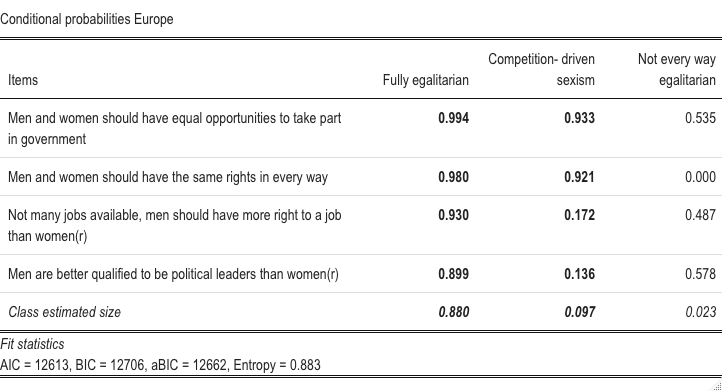
\includegraphics[height=0.4\textwidth]{graphics/prob_eu.png}\\
	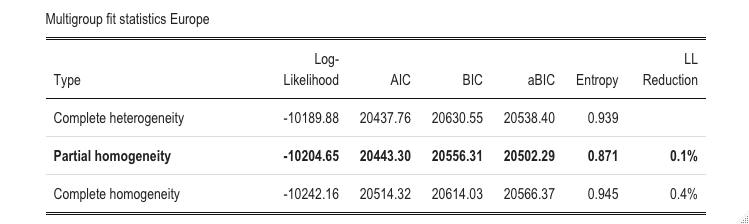
\includegraphics[height=0.2\textwidth]{graphics/mg_eu.png}
\end{figure}
	
\end{frame} 

\begin{frame}{South America - 4 classes}
	
\begin{figure}
	\centering
	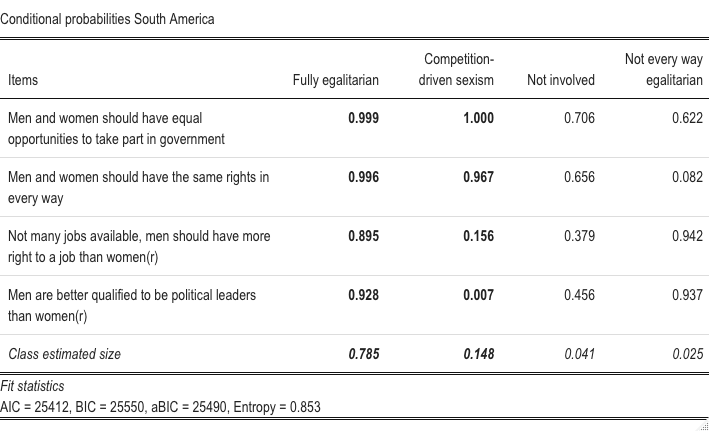
\includegraphics[height=0.4\textwidth]{graphics/prob_la.png}\\
	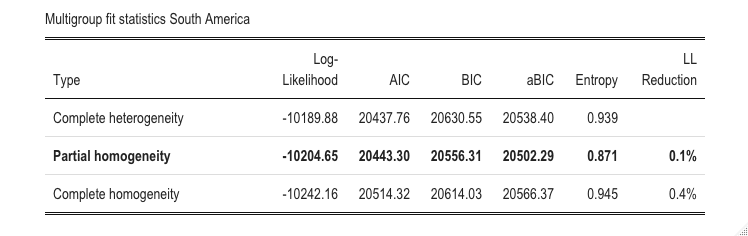
\includegraphics[height=0.2\textwidth]{graphics/mg_la.png}
\end{figure}
	
\end{frame} 


\begin{frame}{Comparability}
	
\begin{figure}
	\centering
	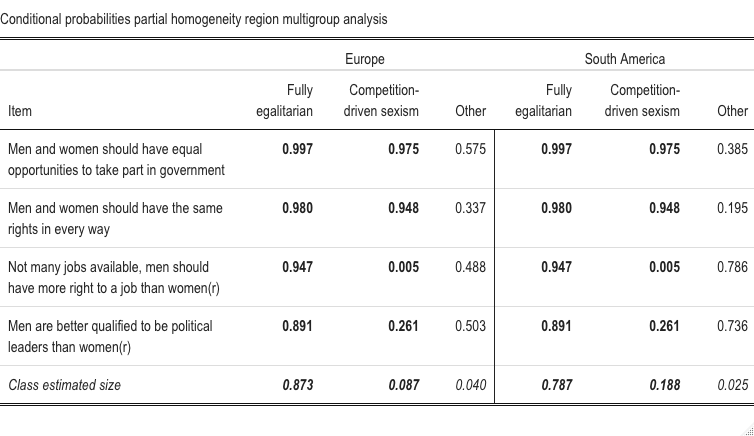
\includegraphics[height=0.4\textwidth]{graphics/prob_reg.png}\\
	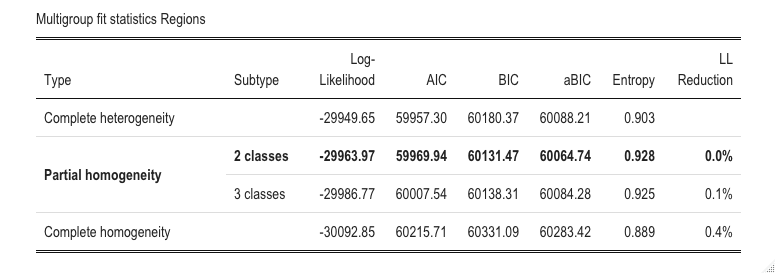
\includegraphics[height=0.2\textwidth]{graphics/mg_reg.png}
\end{figure}
	
\end{frame} 


\section{Further analysis}
%\begin{frame}{Characterization of classes}
%\begin{figure}
%	\centering
%	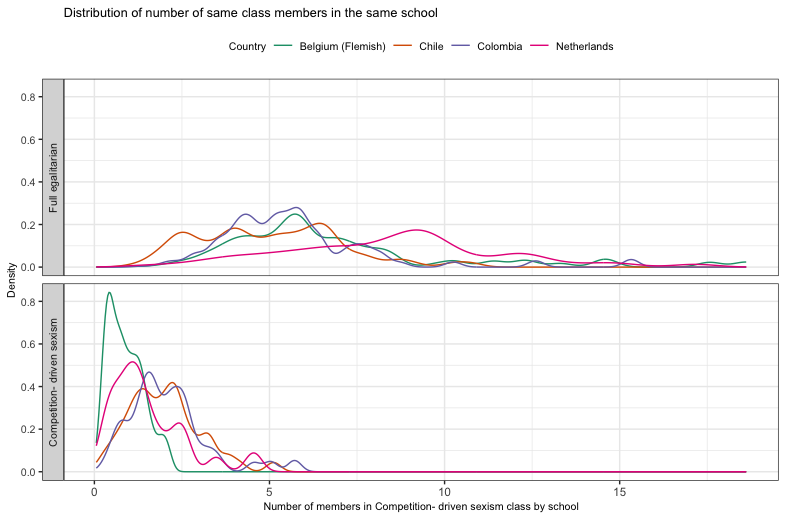
\includegraphics[height=0.6\textwidth]{graphics/schoolsize.png}\\
%\end{figure}
%\end{frame} 
%
%\begin{frame}{Civic knowledge among members}
%\begin{figure}
%	\centering
%	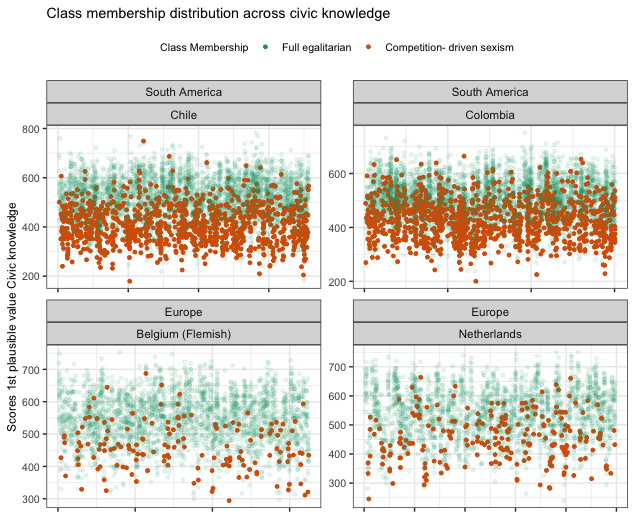
\includegraphics[height=0.6\textwidth]{graphics/civickn.png}\\
%\end{figure}
%\end{frame} 
%
%\begin{frame}{Gender and socioeconomical background}
%\begin{figure}
%	\centering
%	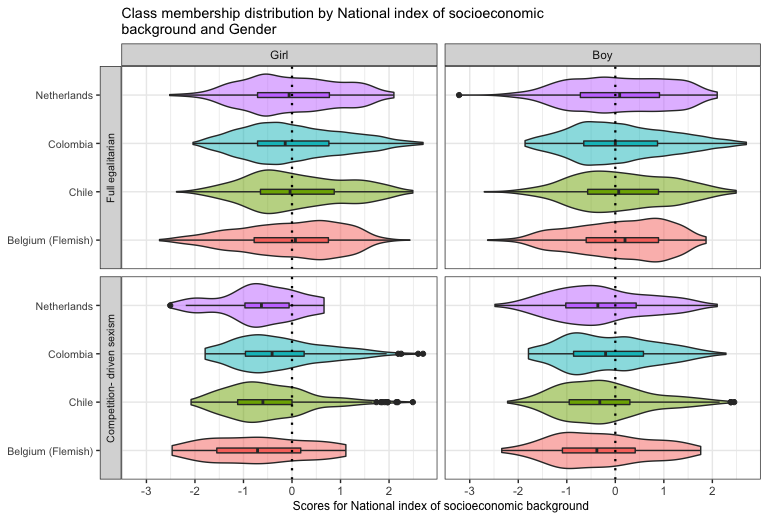
\includegraphics[height=0.6\textwidth]{graphics/gendernisb.png}\\
%\end{figure}
%\end{frame} 
\begin{frame}{Characterization of classes}
\begin{figure}
	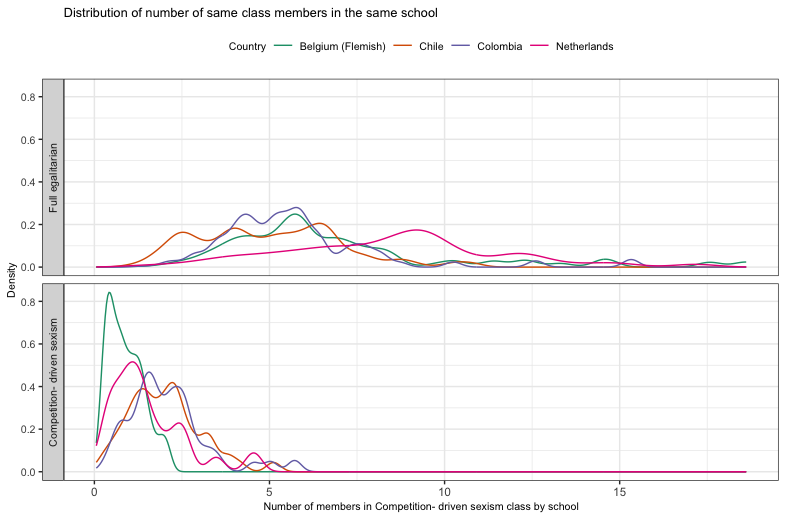
\includegraphics[width=0.4\textwidth]{graphics/schoolsize.png}\\
	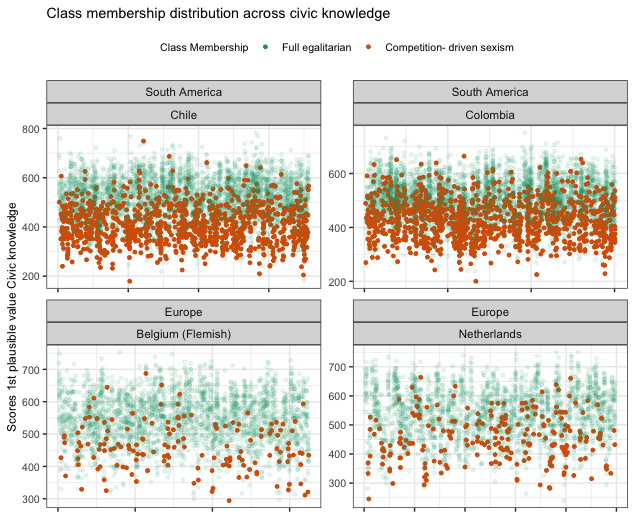
\includegraphics[height=0.3\textwidth]{graphics/civickn.png} 
	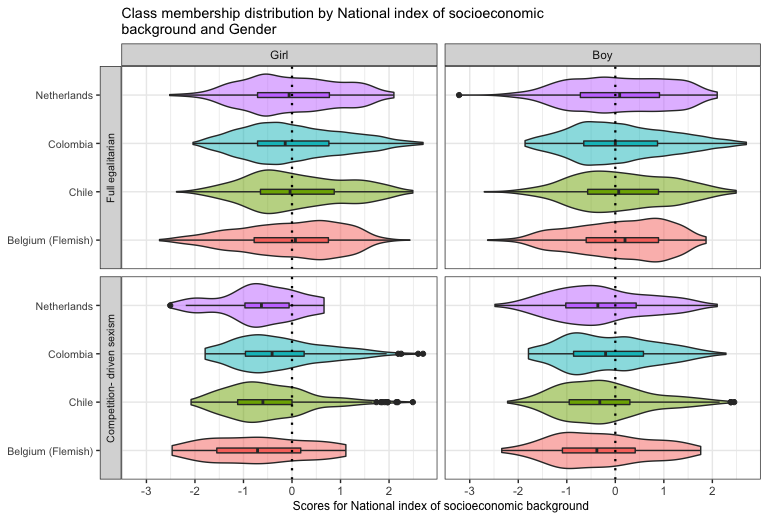
\includegraphics[height=0.3\textwidth]{graphics/gendernisb.png}
\end{figure}
\end{frame} 
\begin{frame}{Logistic regression}
\begin{figure}
	\centering
	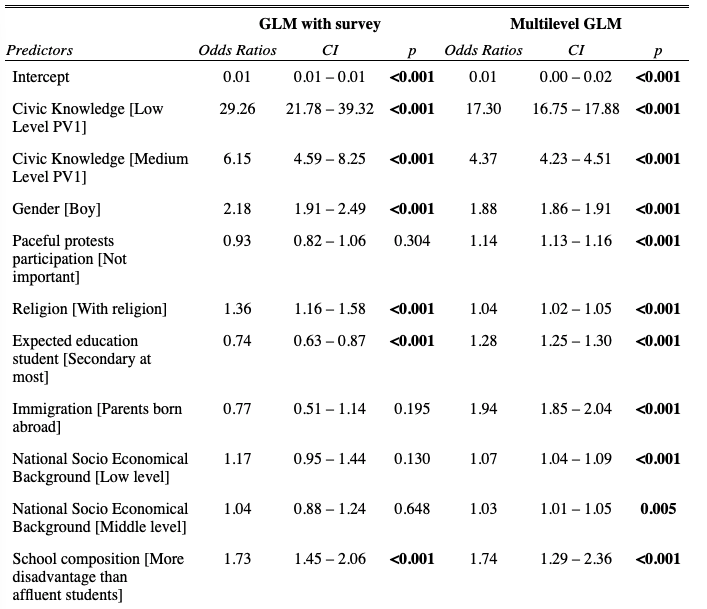
\includegraphics[height=0.4\textwidth]{graphics/logmodels.png}
	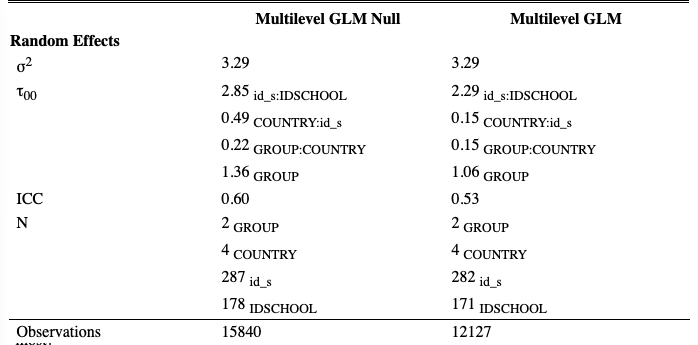
\includegraphics[height=0.2\textwidth]{graphics/re_hlm.png}\\
\end{figure}
\end{frame} 

\begin{frame}{What is next?}
\begin{itemize}

	\item It is possible to include more countries in each group?.
	\item It is possible to include another group (Asia)?.
	\item Identify relevant factors that influence the class membership.
	
\end{itemize}
\end{frame}

\begin{frame}{References}
\Fontvi
\begin{itemize}
\item Agresti, A. (2013). Categorical data analysis (3rd ed).\\

\item Barber, C., \& Ross, J. (2020). Profiles of adolescents’ civic attitudes in sixteen countries\\

\item Davidov, E., Schmidt, P., \& Billiet, J. (Eds.). (2011). Cross-cultural analysis: Methods and applications.\\

\item Hagenaars, J. A., \& McCutcheon, A. L. (Eds.). (2002). Applied latent class analysis (1st ed.). \\

\item Hallquist, M. N., \& Wiley, J. F. (2018). MplusAutomation: An r package for facilitating large-scale latent variable analyses in Mplus. \\

\item Rutkowski, L., Davier, M. von, \& Rutkowski, D. (2014). Handbook of international large-scale assessment background, technical issues, and methods of data analysis.\\

\item Vermunt, J. K. (2014). Latent class model. In A. C. Michalos (Ed.), Encyclopedia of quality of life and well-being research 

\item Wang, J., \& Wang, X. (2020). Structural equation modeling: Applications using mplus (2nd ed.). \\
\end{itemize}
\end{frame} 

\begin{frame}
	\vspace{15mm}
	\begin{center}
Thank you for your feedback!
\end{center}
\end{frame}

\end{document}